\section{Моделирование эксперимента в \er.}
\label{section:simulations}

Другой важной задачей текущей работы является компьютерное моделирование проведённых экспериментов, которое проводилось с помощью программного пакета \er~\cite{er}.
Это вычислительный пакет (фреймворк) для Монте-Карло симуляций откликов детекторов, реконструкции событий и анализа экспериментов проекта EXPERT\footnote{Проект EXPERT является одной из составляющих SuperFRS Experiment Collaboration в NUSTAR@FAIR.}.
Пакет \er\ является одним из продуктов фреймворка FAIRroot~\cite{FAIRroot}, который представляет собой набор инструментов и подходов для создания и конфигурации процедур симуляции, реконструкции и анализа. FAIRroot соединяет функциональность таких широкоиспользуемых инструментов, как ROOT Data Analysis Framework~\cite{root} и GEANT4~\cite{geant}.
\er\ создан по аналогии с другими продуктами FAIRroot (например, CBMRoot~\cite{CBMroot}, PandaRoot~\cite{PANDAroot}) и отличается высокой модулярностью внедренных детекторов.

Для детектора NeuRad используется так называемый метод имитационного моделирования отклика детектора \cite{vitalik}. 
Результатом работы данного метода является форма сигналов на анодах ФЭУ от всех энерговыделений всех волокон в выбранном событии. Сигнал на каждом аноде фотоэлектронного умножителя является суммой сигналов от единичных фотоэлектронов. В дальнейшем этот сигнал используется для формирования временной привязки. Для получения формы сигнала моделируется отклик от каждого фотоэлектрона. Для этого последовательно моделируются следующие процессы:
\begin{enumerate}
	\item Транспорт всех частиц в событии через объём сцинтиллятора и разыгрывание происходящих с ними физических процессов, включающих ядерные и электромагнитные взаимодействия, в частности, потери энергии на ионизацию. Для этого используется инструмент GEANT4 \cite{geant}.
	\item Преобразование энерговыделения на каждом шаге $dE_i$ в величину той же размерности, но пропорциональную количеству рождённого света $dL_i$
	\begin{equation}
	\label{eq:lyield}
	dL_i = Q_i\cdot dE_i,
	\end{equation}
	где $Q_i$ - коэффициент пропорциональности, называющийся квенчинг-фактором. 
	Для расчёта квенчинг-фактора используется модифицированный закон Биркса в форме
	\begin{equation}
	\label{eq:quenching}
	Q_i = \frac{A}{1+B\frac{dE_i}{dx_i}+C\big(\frac{dE_i}{dx_i}\big)^2},
	\end{equation}
	где dx$_i$ - шаг трассировки частицы, на котором произошло энерговыделение dE$_i$; A,B и С - константы Биркса, соответствующие данному материалу \cite{vratislav}.
	\item Для каждого непрерывного участка энерговыделения вычисляются интегральные значения депозита энергии (E), условной величины, пропорциональной количеству света (L), и количеству рождённых фотонов (N$_p$)
	\begin{eqnarray}
	E=\sum E_i;\nonumber \\
	L=\sum L_i;\\
	N_p=L\cdot C_{\rm ly},\nonumber 
	\end{eqnarray}
	где $C_{\rm ly}$ - световыход сцинтиллятора, т.е. количество фотонов, рожденных на один МэВ энергопотерь электрона. Для сцинтиллятора BCF12 использующегося в NeuRad , $C_{ly} = 8000$\,фотонов/МэВ~\cite{crystals},
	причём количество фотонов, испускаемое в определённый момент времени рассчитывается как
	\begin{equation}
	N_p(t) = \frac{N_{0}}{\tau_{d}}\exp\left(\frac{-t}{\tau_{d}}\right),
	\label{scintSHAPE}
	\end{equation}
	где $N_{0}$-общее количество испущенных фотонов, $t$ - время, $\tau_{d}$-параметр высвечивания используемого сцинтиллятора, для BCF12 который равен 3,2\,нс \cite{crystals}. 
	Учитываются две причины зависимости количества фотонов, достигших фотокатода, от продольной координаты точки взаимодействия: телесный угол, под которым виден фотокатод из точки взаимодействия с учетом полного внутреннего отражения, и поглощение света в материале волокна.
	\item Для данного энерговыделения рассчитывается среднее число родившихся на каждом пикселе фотоэлектронов 
	\begin{equation}
	\bar{N}_{pe} = N_p \cdot C_{qe},
	\end{equation}
	где $C_{qe}$ - квантовая эффективность фотокатода \cite{vratislav}. Для фотокатода ФЭУ HM9500 квантовая эффективность равна примерно 20\% \cite{Hamamatsu}.
	Количество родившихся в событии фотоэлектронов разыгрывается по закону Пуассона со средним $\bar{N}_{pe}$.
%%	\item 
%	Моделирования фотоэлектронов, родившихся на фотокатоде. 
%	Для этого необходимо знать время прихода соответствующего фотона на катод и амплитуду родившегося фотоэлектрона, расчёт которых подробно описан в источнике \cite{vitalik}.
	\item
	Амплитуда одноэлектронного сигнала рассчитывается как
	\begin{equation}
	A_{pe}=|N(A,\sigma)|,
	\end{equation}
	где $N(A,\sigma)$ - функция нормального распределения с подобранными параметрами А и $\sigma$.
	А время прихода сигнала на анод
	\begin{equation}
	T_{pe}=T_k+N(D_{\rm PMT},J_{\rm PMT}),
	\end{equation}
	где $D_{\rm PMT}$ - задержка на динодной системе, $J_{\rm PMT}$ - флуктуация времени прохождения электронной лавины через динодную систему, $N(D_{\rm PMT},J_{\rm PMT})$ - функция нормального распределения, $T_k$ - время, за которое фотон достигает фотокатода ФЭУ, двигаясь вдоль оптического волокна детектора. Для ФЭУ, использовавшегося в эксперименте, задержка и флуктуация времени прохождения известны и равны соответственно 6 и 0.4\,нс \cite{Hamamatsu}.
	\item Получив параметры сигналов фотоэлектронов, рассчитывается форма сигнала. Использовалась следующая функция сигнала фотоэлектрона: 
	\begin{equation}
	\label{eq:1electronSIM}
	U(t)=a\, A_{pe}\,(t-T_{pe})^2 \exp\left(- \frac{t-T_{pe}}{b} \right),
	\end{equation}
	где $a$ и $b$ – подбираемые коэффициенты, $U(t)$ - амплитуда сигнала в момент времени t, $A_{pe}$ и $T_{pe}$ - разыгранные время и амплитуда одноэлектронного сигнала. 
	Коэффициенты $a$ и $b$ определяются для данного ФЭУ из эксперимента.
	Получив формы сигналов от каждого фотоэлектрона, определяется суммарный токовый сигнал на аноде как сумму сигналов с каждого фотоэлектрона. 
	Единственным качественным отличием сигналов анода, получаемых с помощью \er\ от экспериментальных, является отсутствие шумовой дорожки и сигналов порождённых космическими лучами.
	
\end{enumerate}

Опции \er\ позволяют создавать модель детектора любой формы и сделанного из любого материала. Была создана виртуальная модель прототипа NeuRad, описанного в главе\,\ref{sec:timeTests}. В геометрии детектора были учтены все свето-изолирующие покрытия и мёртвые слои чувствительных частей детектора. 
Под мёртвым слоем детектора подразумевается  часть детектора, расположенная между наружной поверхностью и чувствительной областью детектора, в пределах которой взаимодействие налетающих частиц с веществом не приводит к возникновению сигналов на выводах детектора.
В виртуальном прототипе детектора NeuRad мёртвый слой равнялся 50\,мкм. Пучок падающих гамма-квантов установленной энергии направлялся с помощью железного коллиматора. Cечение коллимированного пучка было квадратным размерами 3$\times$3 мм$^ 2$, а сам пучок был направлен на середину прототипа, так же, как и в эксперименте.
Схема виртуального эксперимента, воссозданного в \er, изображена на Рис.\ref{ris:sim}. 

\begin{figure}
	\centering
	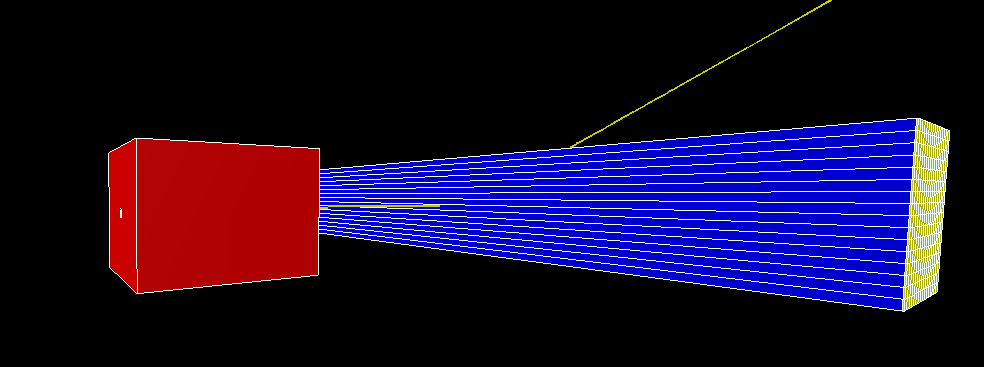
\includegraphics[width=\linewidth]{sim.png}
	\captionof{figure}{Схема виртуального эксперимента в \er. Красным цветом изображён коллиматор, синим - прототип NeuRad, жёлтым - ФЭУ. Красной линией обозначена траектория движения гамма-кванта, одного из разыгранных событий.}
	\label{ris:sim}
\end{figure}

Таким образом записывались формы сигнала из 512 файберов, каждый из которых соответствовал одному аноду ФЭУ. Также, как в эксперименте, из всех моделируемых данных для получения временного разрешения, нам было достаточно сигналов с одного оптического волокна, выбранное посередине пучка.

\begin{figure}[!ht]
	\centering
	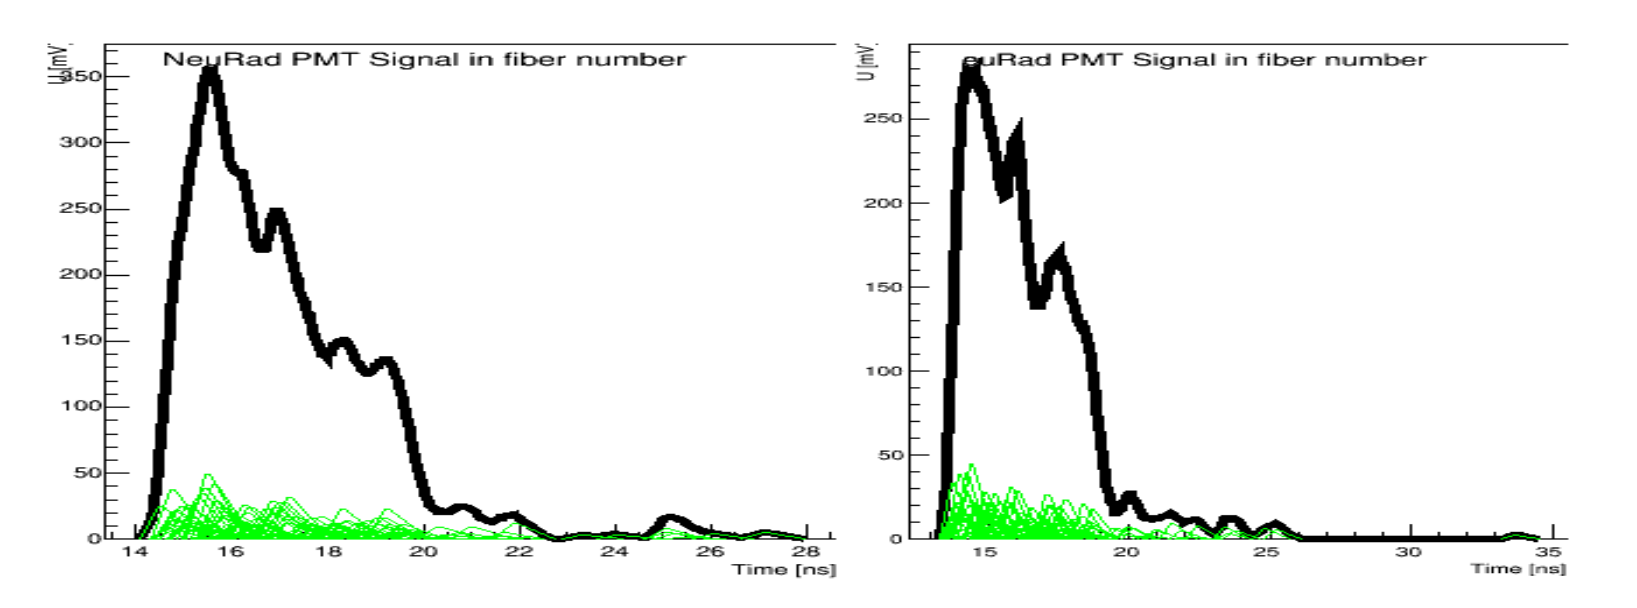
\includegraphics[width=\linewidth]{simsignal.png}
	\captionof{figure}{Сигналы с двух сторон волокна. Сигналы ФЭУ, обозначенные чёрным цветом, образованы суммированием сигналов всех фотоэлектронов, которые изображены зелёным цветом.}
	\label{ris:simsignal}
\end{figure}

Формы сигналов, приходящих с данного волокна на пиксели ФЭУ записывались в файл формата Root \cite{root} при условии, что амплитуда с одной из сторон превысила выбранное значение 30\,мВ. Данное условие записи  сигналов является виртуальной аналогией триггера оцифровывающего устройства, использовавшегося в эксперименте.
Пример результата моделирования формы сигнала с двух сторон одного оптического волокна представлен на Рис.\ref{ris:simsignal}.

Таким образом, с помощью фреймворка \er\ можно получать данные, по структуре схожие с экспериментальными. Поэтому алгоритмы обработки, описанные в следующей главе, применяются и для экспериментальных данных и для моделированных. 
